% This is a general template file for the LaTeX package SVJour3
% for Springer journals. Original by Springer Heidelberg, 2010/09/16
%
% Use it as the basis for your article. Delete % signs as needed.
%
% This template includes a few options for different layouts and
% content for various journals. Please consult a previous issue of
% your journal as needed.
%
\RequirePackage{fix-cm}
%
%\documentclass{svjour3}                     % onecolumn (standard format)
%\documentclass[smallcondensed]{svjour3}     % onecolumn (ditto)
\documentclass[smallextended]{svjour3}       % onecolumn (second format)
%\documentclass[twocolumn]{svjour3}          % twocolumn
%
\smartqed  % flush right qed marks, e.g. at end of proof
%
\usepackage{graphicx}
\usepackage{amsmath}
\usepackage{amssymb}
%
% insert here the call for the packages your document requires
%\usepackage{mathptmx}      % use Times fonts if available on your TeX system
%\usepackage{latexsym}
% etc.
%
% Jag's 
\usepackage{tabu}
\usepackage{cancel}
\usepackage{algorithm}
\usepackage{algorithmicx}
\usepackage{algpseudocode}
%\usepackage[caption=false]{subfig}
\usepackage{subcaption}
\captionsetup{compatibility=false}

\algdef{SE}[DOWHILE]{Do}{doWhile}{\algorithmicdo}[1]{\algorithmicwhile\ #1}%

\DeclareMathOperator{\Order}{{\mathcal O}}

% please place your own definitions here and don't use \def but
% \newcommand{}{}
\newcommand{\bm}[1]{\boldsymbol{#1}}
\newcommand{\mSigma}{\Sigma}
\newcommand{\smallocite}[1]{{\small\ocite{#1}}}
% \newcommand{\bm}[1]{\boldsymbol{#1}}
\newcommand{\dif}[1]{\text{d}{#1}}

\newcommand{\naturals}{\mathbb{N}}
\newcommand{\reals}{\mathbb{R}}
\newcommand{\integers}{\mathbb{Z}}
\newcommand{\complex}{\mathbb{C}}
\newcommand{\hilbert}{\mathbb{H}}

\newcommand{\cf}{\mathcal{F}}
\newcommand{\cx}{\mathcal{X}}
\newcommand{\tcx}{\widetilde{\cx}}

\newcommand{\valpha}{{\bm{\alpha}}}
\newcommand{\vbeta}{{\bm{\beta}}}
\newcommand{\vlambda}{{\bm{\lambda}}}
\newcommand{\vphi}{{\bm{\phi}}}
\newcommand{\vpsi}{{\bm{\psi}}}
\newcommand{\vtheta}{{\bm{\theta}}}
\newcommand{\vthetaMLE}{\bm{\theta}_{\text{MLE}}}
\newcommand{\hvtheta}{\hat{\vtheta}}
\newcommand{\va}{\bm{a}}
\newcommand{\vb}{\bm{b}}
\newcommand{\vc}{\bm{c}}
\newcommand{\vC}{\bm{C}}
\newcommand{\tvc}{\tilde{\bm{c}}}
\newcommand{\vh}{\bm{h}}
\newcommand{\vf}{\bm{f}}
\newcommand{\vk}{\bm{k}}
\newcommand{\vs}{\bm{s}}
\newcommand{\vt}{\bm{t}}
\newcommand{\vv}{\bm{v}}
\newcommand{\vV}{\bm{V}}
\newcommand{\vw}{\bm{w}}
\newcommand{\vW}{\bm{W}}
\newcommand{\vx}{\bm{x}}
\newcommand{\dx}{\dif{{x}}}
\newcommand{\dt}{\dif{{t}}}
\newcommand{\dvx}{\dif{\bm{x}}}
\newcommand{\dvs}{\dif{\bm{s}}}
\newcommand{\dvt}{\dif{\bm{t}}}
\newcommand{\vrho}{\bm{\rho}}
\newcommand{\hy}{\hat{y}}
\newcommand{\vy}{\bm{y}}
\newcommand{\hvy}{\hat{\vy}}
\newcommand{\vz}{\bm{z}}
\newcommand{\dvz}{\dif{\bm{z}}}
\newcommand{\tf}{\tilde{f}}

\newcommand{\tvv}{\tilde{\vv}}
\newcommand{\tvz}{\tilde{\vz}}

\newcommand{\vCvtheta}{{C_\vtheta}}

\newcommand{\hatvy}{\hat{\bm{y}}}
\newcommand{\haty}{\hat{y}}
\newcommand{\tvy}{\tilde{\bm{y}}}
\newcommand{\ty}{\tilde{y}}
\newcommand{\vzero}{\bm{0}}
\newcommand{\vone}{\bm{1}}
\newcommand{\tvone}{\tilde{\bm{1}}}
\newcommand{\mC}{\mathsf{C}}
\newcommand{\mCtheta}{{\mathsf{C}_{\vtheta}}}
%\newcommand{\mCthetaInv}{{\mathsf{C}^{-1}_{\vtheta}}}
%\newcommand{\mCthetaMLE}{{\mathsf{C}_{\vthetaMLE}}}
%\newcommand{\mCthetaInvMLE}{{\mathsf{C}^{-1}_{\vthetaMLE}}}
\newcommand{\mCInv}{{\mathsf{C}^{-1}}}


\newcommand{\tmC}{\widetilde{\mathsf{C}}}
\newcommand{\tlambda}{\tilde{\lambda}}

\newcommand{\mL}{\mathsf{L}}

\newcommand{\mLambda}{\mathsf{\Lambda}}
\newcommand{\mLambdaInv}{\mathsf{\Lambda}^{-1}}

\newcommand{\mV}{\mathsf{V}}
\newcommand{\mW}{\mathsf{W}}

\newcommand{\tvrho}{\widetilde{\vrho}}
\newcommand{\heta}{\hat{\eta}}
\newcommand{\hmu}{\hat{\mu}}
\newcommand{\hnu}{\hat{\nu}}
\newcommand{\rhoCond}{\mathring{\vrho}}

\newcommand{\MLE}{\text{MLE}}
%\newcommand{\errtol}{\text{tol}}
\newcommand{\errtol}{\epsilon}
\newcommand{\errn}{\text{err}_{n}}
\newcommand{\diag}{\text{diag}}

\def\abs#1{\ensuremath{\left \lvert #1 \right \rvert}}
\newcommand{\norm}[2][{}]{\ensuremath{\left \lVert #2 \right \rVert}_{#1}}
\newcommand{\ip}[3][{}]{\ensuremath{\left \langle #2, #3 \right \rangle_{#1}}}

\newenvironment{nalign}{
    \begin{equation}
    \begin{aligned}
}{
    \end{aligned}
    \end{equation}
    \ignorespacesafterend
}

\providecommand{\argmin}{\operatorname*{argmin}}
\providecommand{\argmax}{\operatorname*{argmax}}

\graphicspath{{./figures/}{D:/Mega/MyWriteupBackup/Sep_2ndweek/}}

%
% Insert the name of "your journal" with
% \journalname{myjournal}
%
\begin{document}
\setlength\abovedisplayskip{1pt}
\setlength{\belowdisplayskip}{1pt}

\title{Fast automatic Bayesian cubature
%\thanks{}
}
% Grants or other notes about the article that should go on the front
% page should be placed within the \thanks{} command in the title
% (and the %-sign in front of \thanks{} should be deleted)
%
% General acknowledgments should be placed at the end of the article.

%\subtitle{Do you have a subtitle?\\ If so, write it here}

%\titlerunning{Short form of title}        % if too long for running head

\author{Jagadeeswaran R.         \and
        Fred. J. Hickernell %etc.
}

%\authorrunning{Short form of author list} % if too long for running head

\institute{F. Author \at
              first address \\
              Tel.: +123-45-678910\\
              Fax: +123-45-678910\\
              \email{fauthor@example.com}           %  \\
%             \emph{Present address:} of F. Author  %  if needed
           \and
           S. Author \at
              second address
}

\date{Received: date / Accepted: date}
% The correct dates will be entered by the editor

\maketitle

\begin{abstract}
Automatic cubatures provide approximations to multidimensional integrals that satisfy user-specified error tolerances.  For multidimensional problems, the sampling density is fixed, but the
sample size, $n$, is determined automatically. Bayesian cubature postulates that the integrand is an instance of a stochastic process.
Prior information about mean and covariance of this process is used to form data-driven error bounds.  However, the process of inferring the mean and covariance governing the stochastic process from $n$ integrand values involves computing matrix inverses and determinants,
which are in general time-consuming $O(n^3)$ operations.
Our work employs low discrepancy data sites and matching kernels that lower the  computational cost to $O(n \log n)$.  The confidence interval for the Bayesian posterior error is used to choose $n$ automatically to satisfy the user-defined error tolerance.  This approach is demonstrated using rank-1 lattice sequences and shift-invariant kernels.

%Include keywords, PACS, and mathematical subject classification numbers as needed.

\keywords{Bayesian cubature \and Probabilistic numeric methods \and GAIL}
% \PACS{PACS code1 \and PACS code2 \and more}
% \subclass{MSC code1 \and MSC code2 \and more}
\end{abstract}

\section{Introduction}
\label{intro}
Cubature is defined as the problem of inferring the integral $\mu = \int f(x)dx$ over a multi-dimensional function $f$ where $\mu$ has no simple analytic value. Typically, $f$ is only accessible in the form of a function handle. 
Numerical integration is a key component of many problems in scientific computing, finance, statistical modeling, and machine learning etc.  
One could use Numerical algorithms to estimate quantities that can not be directly computed, using the results of more readily available computations.


%Multivariate integrals arise in applications such as evaluating financial risk, computing multivariate probabilities, statistical physics, and uncertainty quantification.


We are interested in finding the integral $\mu : \mathcal{F} \to \mathbb{R}$ of $f$ of the form:

\begin{equation}
\label{eqn:defn_mu}
\mu(f) := \mathbb{E}[f(\bm{X})] := \int_{\mathcal{X}} f(\vx)\, \nu(\dif\vx),
\end{equation}
which is approximated by a cubature algorithm $\hmu : \mathcal{F} \to \mathbb{R}$, where
\begin{equation}
\label{eqn:defn_hmu}  % remove this
\hmu(f) := w_0 + \sum_{i=1}^{n} f(\vx_i) w_i = \int_{\mathcal{X}} f(\vx)\, \hat{\nu}(\dif\vx),
\end{equation}
where $\nu$ is the probability measure and $\hat{\nu}$ is the sampling measure and the function $f$ has domain $\mathcal{X} \subseteq \mathbb{R}^d$. 
Here $f$ is the given black-box function that provides $f(\vx)$ for any $\vx \in \mathcal{X}$.
After perhaps a transformation of integration variable, one may pose any problem as constructing an accurate approximation to the unit cube $\mathcal{X} = [0,1]^d$. 
The weights $\vw = \{w_i\}_{i=0}^n$ and nodes $\{x_i\}_{i=1}^n$ are typically chosen to minimize the integral approximation error $\abs{\mu(f) - \hmu(f)}$.



Traditional cubature methods assume the integrand to be a deterministic function.
An alternative to this approach is to assume that the integrand is a \emph{stochastic process}.
Bayesian cubature (BC) methods assume the integrand is an instance of a Gaussian process. 
BC methods approximate the multivariate integrals that cannot be evaluated analytically, using weighted sums of integrand values at carefully chosen nodes over the domain $\mathcal{X}$ as shown in eqn  (\ref{eqn:defn_hmu}).


%Multivariate integrals evaluation by QMC methods is an important problem studied by Ian Sloan. 



Traditional cubature methods may not provide any guaranteed error accuracy. 
%Though the QMC methods are known to have convergence rate of $\Order(n^{-(1-\delta)})$, this information is not sufficient to identify the number of samples $n$ required to meet the given error tolerance, $\errtol$. 
The goal of this work is to develop a guaranteed, BC algorithm using the confidence intervals given by Bayesian posterior error. 
Our algorithm strives to find the minimum sample size `$n$' - \textit{number of integrand values} required so that the error $\abs{\mu(f) - \hmu(f)}$ is less than the user-defined error threshold $\errtol$, i.e, 
\[
\abs{\mu(f) - \hmu(f)} \leq \errtol 
\] 
But the true error $\abs{\mu(f) - \hmu(f)}$ will not be available for problems that do require cubature methods.
So we compute an approximate error bound $\errn$ using the confidence interval obtained from the posterior error which meets,
\begin{align*}
\errn \leq \abs{\mu(f) - \hmu(f)}
\end{align*}
By calculating a data-driven error bound, our algorithm adaptively determines `$n$'.
An added advantage of our approach is being data-driven, so it does not require any other parameter of the integrand like the `total variation'.
%To minimize the integration error $\errn$, one can appeal to loss functions based on the \textit{posterior error distribution} given the observed function values.


%Probability theory can be used to quantify \emph{epistemic} uncertainty arising from the missing information. 
The ``algorithms for numerical tasks" that return uncertainties in their calculations are called \emph{probabilistic numeric methods}. %Uncertainties could arise from the loss of precision induced by numerical calculation with limited time or hardware.
Our BC algorithm can be categorized as a probabilistic numeric method, due to the nature of assumptions made and the confidence interval it provides.

Section 2 introduces the Bayesian approach to estimate the posterior error and develops the concepts to derive error bound. Then formulates the Automatic cubature algorithm using the error bound. Finally demonstrates why directly using Bayesian cubature algorithm is computationally very expensive.
Section 3 Introduces the concept of �Fast transform kernel� and develops the concepts to make the Bayesian cubature faster which is the major contribution of this research.
Section 4 Demonstrates the realization of �Fast transform kernel� using a shift-invariant kernel and Rank-1 Lattice points.
Section 5 covers further enhancements to the algorithm to avoid cancellation error and make it faster. Finally, numerical examples are shown using the faster algorithm developed.




\section{Bayesian cubature}
\label{sec:1}
%Text with citations \cite{RefB} and \cite{RefJ}.

This section introduces the concepts of the Bayesian cubature and derives all the basic results which will be used in the next section for further speedup of the algorithm. \emph{Bayesian posterior error} \cite{Fred2017} is used to estimate an error bound for the cubature. 

\subsection{Bayesian posterior error}
\label{sec:2}

\iffalse
as required. Don't forget to give each section
and subsection a unique label (see Sect.~\ref{sec:1}).
\paragraph{Paragraph headings} Use paragraph headings as needed.
\begin{equation}
a^2+b^2=c^2
\end{equation}
\fi


Random $f$ postulated by Diaconis \cite{DiaconisBayesian}, O'Hagen \cite{HagenBayes}, Ritter \cite{RiterAverage}, Rasmussen and Ghahramani \cite{RasmussenBayesian} and others: $f \sim \mathcal{GP}(m,s^2 C_\vtheta)$, a Gaussian process from the sample space $\mathcal{F}$ with mean $m$ and covariance function $s^2C_\vtheta$, $C_\vtheta: \mathcal{X} \times \mathcal{X} \to \mathbb{R} $. In this work, we use $\mathcal{X} = [0,1]^d$ and uniform measure.  The scale parameter $s^2$ and shape parameter $\vtheta$ should be estimated.

For a Gaussian process, all vectors of linear functionals of $f$ have a multivariate Gaussian distribution. Sometimes we drop $\vtheta$ in the writings to simplify the notation. With this assumption,
\begin{align*}
\label{eqn:kernel_integral_definitions}
\begin{array}{cc}
\mu(f) \sim \mathcal{N}(m \mu(1), s^2 c_0), 
\quad
c_0 = \int_{[0,1]^2} C_\vtheta(\vx,\vt) \, \dif{\vx} \, \dif{\vt},
\\
\vf  = \left( f(\vx_i)\right)_{i=1}^n \sim \mathcal{N}(m \vone, s^2 \mC), 
\quad
\mC = \left(  C_\vtheta(\vx_i,\vx_j)  \right)_{i,j=1}^n,
\\
\hmu(f) = w_0 + \vw^T \vf \sim \mathcal{N} (w_0 + m \vw^T \vone, s^2 \vw^T \mC \vw),
\quad
\vone = \left(1,...,1 \right)^T.
\end{array}
\end{align*}

Let us consider a fixed node set design $\{ \vx_i \}_{i=1}^n$, then we observe $\vy = \{y_i = f(\vx_i) \}_{i=1}^n$. With this, the conditional probability density of error $\mu-\hmu$ given observed data $\vy$:
\begin{nalign}
\mu-\hmu\;|\vy
\; \sim \; \mathcal{N} 
\left(
\begin{array}{cc}
-w_0 + m (\mu(1) - \vone^T  \mC^{-1}\vc )
+
\vy^T( \mC^{-1}\vc - \vw ),
\\
s^2 (c_0 - \vc^T\mC^{-1}\vc) 
\end{array}
\right),
\end{nalign}
\begin{align*}
\text{where} \quad 
\vc = \left( \int_{[0,1]} C_\vtheta(\vx_i,\vx) \dif{\vx} \right)_{i=1}^n
\end{align*}
By choosing the weights $w_0$ and $\vw$ carefully:
\begin{align*}
w_0 =  m (\mu(1) - \vone^T  \mC^{-1}\vc ),
\quad
\vw = \mC^{-1}\vc,
\end{align*}
we can force the posterior error $\mu-\hmu\;|\vy$ to have zero mean:
\begin{align*}
\label{eqn_error_cond_prob}
\mu-\hmu\;|\vy
\; \sim \; \mathcal{N} 
\left(
0, \;
s^2 (c_0 - \vc^T\mC^{-1}\vc) 
\right)
,
\end{align*}
which leads to unbiased solution:
\begin{align*}
\begin{array}{cc}
\hmu(f) = w_0 + \vw^T \vy = 
m(\mu(1) - \vone^T  \mC^{-1}\vc )
+
\vc^T \mC^{-1} \vy
\end{array}
\end{align*}
If we can assume the observed data comes from the source of Gaussian process with zero mean $m=0$ then $w_0 = 0$; This fact can be used where applicable. For the integration problem as defined eqn (\ref{eqn:defn_mu}), which is the focus of this work, $\mu(1) = 1$. So, further in this work, we use the actual value.

Subsequently, since the posterior error $\mu-\hmu\;|\vy$ is a Normal random variable, we can obtain a confidence interval or inference using integrand-samples and estimated-parameters. If $n$ is chosen large enough to make
\begin{align}
%\label{eqn_stopping_criterion_1}
\errn := 2.58 \; \sqrt{ s^2 (c_0 - \vc^T\mC^{-1}\vc) } \leq \errtol
\end{align}
Then
\begin{align}
\label{eqn_prob_confidence_interval}
\mathbb{P}_f \left[
|\mu-\hmu| \leq \errtol
\right] \geq 99\%
\end{align}
where the constant $2.58$ comes from the fact that $99\%$ standard Normal distribution is comprised within $2.58$ times the standard deviation. We call $\errn$, error bound and $\errn \leq \errtol$, stopping criterion.















\subsection{Maximal likelihood estimation of parameters}
The covariance scale parameter $s^2$, mean $m$ and kernel shape parameter $\vtheta$ must be estimated. We choose to do this estimation through Maximum likelihood estimation (MLE), by using the observed integrand values for the purpose of estimating the integral.  The log-likelihood function of the parameters given the data $\vy = \{y_i = f(\vx_i)\}_{i=1}^n$ is 
\begin{nalign}
& l(s,m,\vtheta | \vy) = \log 
\left(
\frac{
\exp\left( -\frac{1}{2} s^{-2} (\vy-m\vone)^T\mCInv(\vy-m\vone)\right) }
{\sqrt{(2\pi)^n \det(s^2\mC)}}
\right) 
\\
&= -\frac{1}{2} s^{-2} (\vy-m\vone)^T\mCInv(\vy-m\vone) - \frac{1}{2} \log(\det\, \mC) - n \log(s ) + \text{constants.}
\end{nalign}

Maximizing $l(s,m,\vtheta | \vy)$ with respect to $m$, provides the MLE of $m$ 
\begin{align}
\label{eqn_m_MLE}
m_\MLE &= \frac{\vone^T \mCInv \vy }{ \vone^T \mCInv \vone}
\end{align}
Then using the above result
\begin{align*}
(\vy-m\vone)^T\mCInv(\vy-m\vone) 
& = 
\vy^T\mCInv\vy - \frac{\vy^T \mCInv \vone \vone^T \mCInv \vy}{\vone^T\mCInv \vone}
\\
& = \vy^T 
\left[ 
\mCInv - 
\frac{ \mCInv \vone \vone^T \mCInv }{\vone^T\mCInv \vone}
\right] \vy.
\end{align*}

Maximizing $l(s,m,\vtheta | \vy)$ with respect to `$s$' provides the MLE of $s$
\begin{align}
\label{eqn_s2_MLE}
\nonumber
s^2_{\MLE}  
&= \frac{1}{n} (\vy-m_{\MLE}\vone)^T\mCInv(\vy-m_{\MLE}\vone) 
\\
&= 
\frac{1}{n}
\vy^T 
\left[ 
\mCInv - 
\frac{ \mCInv \vone \vone^T \mCInv }{\vone^T\mCInv \vone}
\right] \vy
\end{align}

Plug in the results of $m_\MLE$ and $s_\MLE$ to simplify the log likelihood:
\begin{align*}
l(s,m,\vtheta | \vy) 
= -\frac{1}{2} n - \frac{1}{2} \log(\det\,\mC) - n \log(s_\MLE) + \text{const}
\end{align*}
By minimizing the negative of $l(s,m,\vtheta | \vy) $ with respect to `$\vtheta$', the MLE of $\vtheta$ can be obtained. This is usually done by numerically searching for the minimum:
\begin{nalign}
\label{eqn_MLE_loss_function}
\vtheta_\MLE
= 
\argmin_{\vtheta}
\left[
 \frac{1}{2n} \log(\det\, \mC) + 
 \log\left(s_\MLE \right) 
\right].
%\argmin_{\vtheta}
%\left[ 
% \log\left(\frac{ (\vy-m_{\MLE}\vone)^T{\mC}^{-1}(\vy-m_{\MLE}%\vone) }{ [\det( \mC^{-1})]^{\frac1n} } \right) 
%\right]
\end{nalign}

\iffalse
The posterior error mean (\ref{eqn_error_cond_prob}) can be simplified using the MLE of mean $m$.
\begin{nalign}
\label{eqn_error_cond_prob_1}
\mu-\hmu|\vy 
& \sim \mathcal{N} 
\left(m (1 - \vone^T  \mC^{-1}\vc )
+
\vy^T( \mC^{-1}\vc - \vw ), s^2 (c_0 - \vc^T\mC^{-1}\vc) \right)
\end{nalign}
where the mean term is rewritten
\begin{align*}
m (1 - \vone^T  \mCInv\vc ) + \vy^T( \mCInv\vc - \vw )
= \vy^T \left( 
\left[
\frac{ (1 - \vone^T  \mCInv\vc ) }{ \vone^T \mCInv \vone}   \mCInv \vone +  \mCInv\vc  \right]- \vw
\right)
\end{align*}
This results shows, if the weights $\vw$ are chosen carefully, as given below, will lead to unbiased posterior error
\begin{align}
\vw =
\frac{ (1 - \vone^T  \mCInv\vc ) }{ \vone^T \mCInv \vone}   \mCInv \vone +  \mCInv\vc  
\end{align}
If we can assume the observed data comes from the source of Gaussian process with zero mean $m=0$, then the weights $\vw$ can be computed as below, to have an unbiased error:
\begin{align}
\vw = \mCInv\vc ,
\end{align}
these results will be used in further computations.
Now using MLE estimated parameters, one can rewrite the error interval in a computable form
\begin{align}
\mathbb{P}_f \left[
|\mu-\hmu| \leq 
2.58 \; 
\sqrt{
s^2_\MLE
 \left(c_{0,\vtheta_\MLE} - {\vc}_{\vtheta_\MLE}^T\mCInv\vc_{\vtheta_\MLE}
\right)
}
\right] = 99\%
\end{align}
Where $s^2_\MLE$ is from the eqn (\ref{eqn_s2_MLE}). Using this, one can define the error bound for Bayesian cubature algorithm.
\fi

Using those two MLE results of $m$ and $s$, the simplified stopping criterion becomes:
\[
2.58 \; \sqrt{ 
\frac{1}{n}
\vy^T 
\left[ 
\mCInv - 
\frac{ \mCInv \vone \vone^T \mCInv }{\vone^T\mCInv \vone}
\right] \vy
(c_0 - \vc^T\mC^{-1}\vc) }  \leq \errtol .
\]

When computing $\hmu$, we use the MLE estimated parameters $m_\MLE , s_\MLE$ and $\vthetaMLE$:
\begin{align*}
\hmu(f) = w_0 + \vw^T \vy = 
m_\MLE(1 - \vone^T  \mC^{-1}\vc )
+
\vc^T \mC^{-1} \vy
\end{align*}































\subsection{Formulating the Bayesian cubature algorithm}
\label{sec:bayes_cubature_algo}
Let the function to integrate be $f \sim \mathcal{GP}(m,s^2 C_\vtheta)$.
Our goal is to compute $\hat{\mu}$ within the error tolerance $\errtol$, i.e.,
\begin{align*}
|\mu - \hat{\mu}| \leq \errtol.
\end{align*}
It is not possible to know true error $|\mu - \hat{\mu}|$ for real problems. So, the error-bound $\errn$ is used as the approximate error estimate.
Our algorithm keeps adding more function values till the stopping criterion is met, i.e., $\errn \le \errtol$. 
Once the stopping criterion is met, the approximation of $\mu$ can be computed:
\begin{nalign}
\label{eqn_muhat}
\hmu_n &= w_0 + \vw^T \vy
 &=
\left(
\frac{ (1 - \vone^T  \mCInv\vc ) }{ \vone^T \mCInv \vone}   \mCInv \vone +  \mCInv\vc 
\right)^T \vy
\end{nalign}
Where the suffix $n$ is used to imply the number of integrand-samples used. In every iteration of the \emph{automatic cubature algorithm (\ref{algorithm1})}, only need to estimate the MLE $\vtheta_\MLE$ and then use it to compute $\mC$ and $\errn$. 



























The following pseudo-code briefly explains the working of Automatic cubature algorithm.
\begin{algorithm}[H]
\caption{}\label{algorithm1}
  \begin{algorithmic}[1]
    \Procedure{AutoCubature}{$f,\errtol$} \Comment{Integrate within the error tolerance}
      \State $n_0 \gets 2^8$ \Comment{start with minimum number of points}
      \State $n \gets n_0, \; n' \gets 0$
      \While{true} \Comment{Iterate till error tolerance is met}
        \State Generate $\{ \vx_i\}_{i=n' + 1}^{n}$ and sample $\{f(x_i)\}_{i=n'+1}^{n}$
        \State Compute error bound \emph{$\errn$ } \Comment{$\errn$ data driven error bound}
        \If{\emph{$\errn \leq \errtol$}}
	        \textbf{break}
        \EndIf
        \State $n' \gets n, n\gets 2 \times n'$
      \EndWhile
      \State Compute cubature weights $\{ w_i \}_{i=1}^{n}$
      \State Compute approximate integral  $\hmu_n$
      \State \textbf{return} $\hmu_n$ \Comment{Integral estimate $\hmu_n$}
    \EndProcedure
  \end{algorithmic}
\end{algorithm}
The main idea behind our algorithm is to continue the iteration loop till the stopping-criterion is met, i.e., $\errn$ is smaller than error threshold $\errtol$. 
At the end of every iteration, if the computed error bound  $\errn$ is higher than the required $\errtol$, algorithm doubles the number of points $n$ and repeats. When the error tolerance $\errtol$ is met, exits the loop. Finally using the $n$ and the MLE estimated parameters, computes the $\hmu_n$.
Hence accurately computing the data-driven error bound $\errn$ which closely matches the true error is very important for the effectiveness of \emph{Automatic cubature algorithm}. Accurate and faster computation of $\errn$ and $\hmu_n$ are the main objective of the following sections.



















\subsection{Example with Matern kernel}


We would like to demonstrate and test numerical accuracy and computational cost of the \textit{Bayesian cubature algorithm} using the results obtained so far.
For this example, we use the Matern kernel:
\begin{align}
\label{matern_kernel}
C_{\vtheta}(\vx, \vt) = \prod_{k=1}^d \exp(-\theta_k|\vx_k-\vt_k|)(1+\theta_k |\vx_k-\vt_k|)
\end{align}



\begin{figure}[htp]
\captionsetup[subfigure]{labelformat=empty}
\centering
\begin{subfigure}[b]{0.49\textwidth}
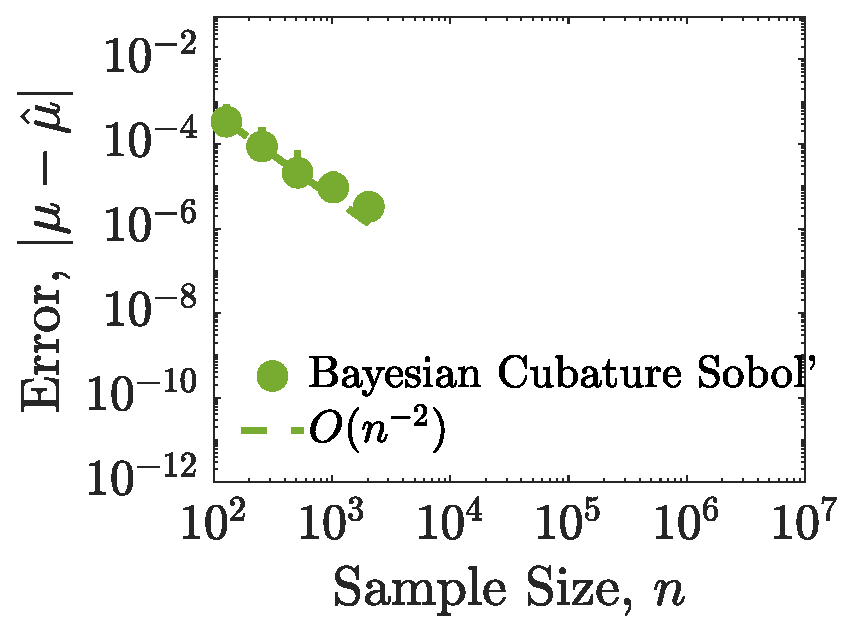
\includegraphics[height=4cm]{MVNBayesianWtSobol}
\end{subfigure}
\centering
\begin{subfigure}[b]{0.49\textwidth}
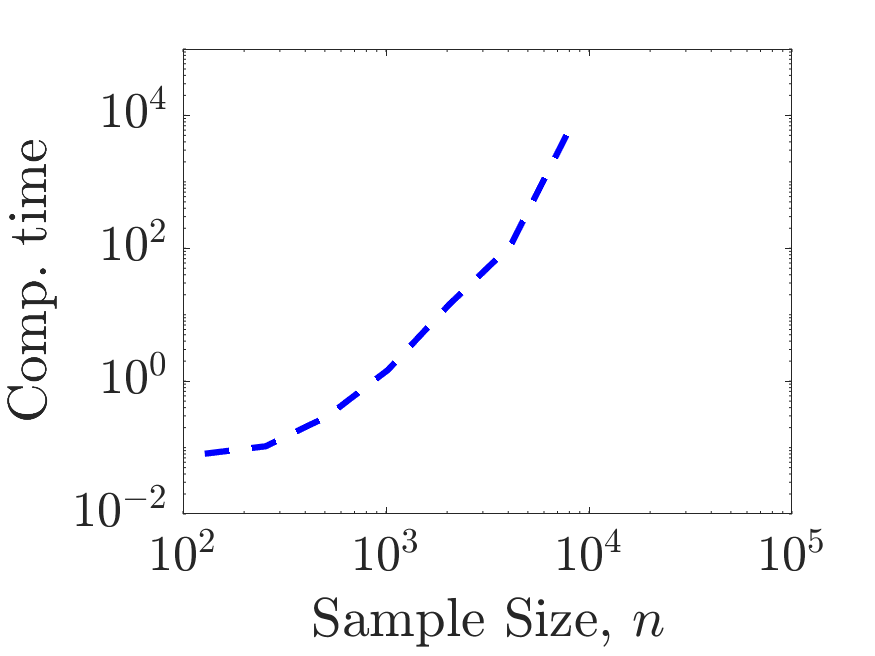
\includegraphics[height=4cm]{MVN_bayesianCubaturecomputeTime}
\end{subfigure}
\caption{MVN for d=2 with Matern kernel  }
\label{fig:MVN_Metern_d2b2}
\end{figure}
While testing on a computer with Intel i7 3630QM and 16GB RAM memory, it took 118 minutes to compute the $\hmu_n$ with $n=2^{13}$. As shown in Figure \ref{fig:MVN_Metern_d2b2}, the time to compute increases rapidly with $n$. 
Especially, the Maximum-likelihood-estimation which needs the computation of loss function is the most time consuming of all. 
Because the loss functions need to computed multiple times, in every iteration to choose the optimal shape parameter which minimizes the loss function. 
It is not only complexity increase, the kernel matrix become highly ill-conditioned with the increasing $n$ number of data-points.
We must use alternative techniques to overcome this problem.
So the \textit{Bayesian cubature} algorithm in the current form is not usable for any practical applications.








































































\section{Fast automatic Bayesian cubature}\label{fast_transform_kernel}
{Bayesian cubature algorithm} described (Section \ref{sec:bayes_cubature_algo}) is very slow due to its computationally intensive nature. This could be a hindrance in real world applications when a larger number of data points are needed. This section and further sections explore techniques to make it faster.

Bayesian cubature algorithm uses the error bound $\errn$ to decide when to stop, and uses MLE loss function (\ref{eqn_MLE_loss_function}) to find the optimal {shape parameter}.
These computations involve covariance matrix inversions and multiplications, which are time-consuming and prone to numerical error. 
When the algorithm tries to adapt by increasing $n$ to get better accuracy, the covariance matrix size also grows, along with it, the matrix condition number also grows significantly causing numerical error in matrix operations. This phenomenon is called ill-conditioning.

One approach to overcome these issues could be to use an efficient method to compute the whole equation without incurring the ill-conditioning, which involves, for example, using \textit{stable computation} \cite{FassBook2007} of the power function. But it is still slower and time-consuming. 

Another approach for stable and faster computation is, using a carefully chosen kernel with some special properties which leads to faster matrix operations, like faster matrix inversion and multiplication. 
This approach is faster in computation while avoiding the numerical error due to ill-conditioning. 
The later approach is the major objective of this research work. 
Our approach is especially to choose a special form of kernel, which is called \emph{fast transform kernel} along with suitable pointset, that will avoid expensive matrix operations.






\subsection{Fast transform kernel}
Suppose the domain is $\mathcal{X} = [0,1]^d$ and the probability measure is uniform, If the kernel $C_\vtheta(\vx,\vt)$ is chosen carefully along with appropriate point set $\{\vx_i\}_{i=1}^n$ have the special properties, so the resulting Gram matrix has factorization of the form:
\begin{align}
\label{eqn:ftk_factor}
\mC &= \Big(C_\vtheta(\vx_i,\vx_j)\Big)_{i,j=1}^n  = (\vC_1,...,\vC_n) 
\\
\nonumber
&= \frac 1n \mV \mLambda \mV^H  = \frac 1n \mV^* \mLambda \mV^T , 
\quad \quad \mV^H = n \mV^{-1},
\end{align}
Where $V^H$ is the Hermitian of $V$,
\begin{gather*}
%\begin{array}{cc}
%\displaystyle
%\label{eqn:ftk_factor_2}
\mV = (\vv_1,...,\vv_n)^T = (\vV_1,...,\vV_n), \; \text{also} \;  \vv_1 = \vV_1 = \vone
\\
\mLambda = \diag(\vlambda), \; 
\vlambda = (\lambda_1, ... \lambda_n),
\\
\mV^{-1} = \frac 1n \mV^H, \;
\mCInv  = \frac 1n \mV \mLambda^{-1} \mV^H
 = \frac 1n \mV^* \mLambda^{-1} \mV^T
%\end{array}
.
\end{gather*}

Suppose the transform $\hat{\vz} = \mV^T \vz$ for any arbitrary $\vz$ can be computed within the computational cost of $\Order( n \, log\, n)$, we call it a \emph{Fast transform}. Consequently $C_{\vtheta}$ is called a \emph{fast transform kernel}.
We use the notation $\hat{\vz}$ to indicate the transform.
The properties of fast transform can be leverage to make the computations in Bayesian cubature algorithm faster. $\vlambda$ can be computed faster by simply,
\begin{align}
\label{eqn:fast_trasnform_to_eigvalues}
\mV^T \vC_1 = \mV^T \left( \frac 1n \mV^* \mLambda \vv_1 \right) =
\underbrace{\left( \frac 1n \mV^T  \mV^* \right) }_{\mathsf{I}} \mLambda \vv_1  =  \mLambda \vone =
\begin{pmatrix}
\lambda_1 \\ \vdots \\ \lambda_n
\end{pmatrix} = \vlambda
\end{align}
Most of our computations are of the form $\va^T\mCInv\vb$, can be simplified easily:
\begin{align*}
\mC V_1 &= \lambda_1 V_1 , \quad \text{by definition}
\\
\mCInv \vone &= \mCInv V_1 = \frac{V_1}{\lambda_1} = \frac{\vone}{\lambda_1} , \quad \text{similarly},
\\
\va^T\mCInv\vb &= \frac 1n \va^T \mV \mLambdaInv \mV^H \vb
= \frac 1n \widehat{\va}^T\mLambdaInv \widehat{\vb}^*
= \frac 1n \sum_{i=1}^n \frac{\widehat{a_i} \widehat{b_i^*}}{\lambda_i}
\end{align*}
where $\widehat{\va} = \mV^T \va$ and $\widehat{\vb} = \mV^T \vb$. Similarly some of the recurring terms in our algorithm are simplified,
\begin{align*}
\vone^T\mCInv\vone &= \vone^T \left(\frac{\vone}{\lambda_1}\right) = \frac{n}{\lambda_1}
\\
\vone^T\mCInv\vy &= \vone^T \left( \frac{\vy}{\lambda_1} \right) = \frac{\sum_{i=1}^n y_i}{\lambda_1} = \frac{\widehat{y_1}}{\lambda_1}
\\
\vy^T\mCInv \vy &= \frac 1n \sum_{i=1}^n \frac{\abs{\widehat{y_i}}^2}{\lambda_i}
\\
\vc^T\mCInv \vone &= \vc^T \left(\frac{ \vone }{\lambda_1} \right) = \frac{\widehat{c}_1}{\lambda_1}
\\
\vc^T\mCInv \vc &= \frac 1n \sum_{i=1}^n \frac{\abs{\widehat{c}_i}^2}{\lambda_i}
\end{align*}
Then the MLE estimates can be simplified using these results:
\begin{align*}
m_\MLE &= \frac{\vone^T\mCInv\vy}{\vone^T\mCInv\vone} = \frac{\widehat{y}_1}{n} = \frac 1n \sum_{i=1}^n y_i
\\
s^2_\MLE &= \frac 1n \vy^T \left[ \mCInv - \frac{\mCInv \vone \vone^T \mCInv}{\vone^T\mCInv\vone}\right]
=
\frac 1n \sum_{i=1}^n \frac{\abs{\widehat{y_i}}^2}{\lambda_i} - \frac{\abs{\widehat{y}_1}^2}{n \lambda_1} = 
\frac 1n \sum_{i=2}^n \frac{\abs{\widehat{y_i}}^2}{\lambda_i}
\end{align*}













\iffalse
\subsection{Computing $s^2_\MLE$ and $m_\MLE$ faster}
In all the computations of Bayesian cubature, $s^2_\MLE$ is used extensively. As a first step, we simplify this to make it faster

\begin{align*}
s^2_\MLE &= \frac{1}{n} (\vy-m_{\MLE}\vone)^T{\mC}^{-1}_\MLE(\vy-m_{\MLE}\vone) 
\\
&=
\frac{1}{n}  \left(
\vy^T{\mC}^{-1}_\MLE \vy  + m_{\MLE}^2 \vone^T{\mC}^{-1}_\MLE \vone
 -2  m_{\MLE}\vone^T{\mC}^{-1}_\MLE\vy
\right) 
\end{align*}
each term in this equation can be simplified further. Further discussions will show the ways to avoid expensive matrix multiplications and inversions in $s^2_\MLE$.






\subsubsection{Computing $\vy^T \mCInv \vy$ :}
The matrix inversion in this term can be avoided by using the property of $\mCtheta = \frac 1n \mV \mLambda \mV^H$ as given in eqn (\ref{eqn:ftk_factor}).
\begin{nalign}
\label{eqn_RKHS_norm}
\vy^T \mCInv \vy &= \vy^T \big(\frac 1n \mV \mLambda \mV^H \big)^{-1} \vy 
 &= \vy^T \big(n \mV^{-H} \mLambda^{-1} \mV^{-1} \big) \vy 
 \\
 & =  \vy^T  n \frac 1n \mV \mLambda^{-1} \frac 1n \mV^H \vy 
 & = \frac 1n \underbrace{ (\mV^T \vy)^T }_{\hatvy^T}  \mLambda^{-1} \underbrace{(\mV^T \vy)^*}_{\hatvy^*} \\
 & = \frac 1n \sum_{i=1}^{n} \frac{|\haty_i|^2}{\lambda_i}
\end{nalign}
where $\hatvy$ is considered to be the \textit{Fast Transform} of $\vy$. i.e., $ \hatvy = W^T y $


















\subsubsection{Computing $\vone^T{\mCtheta}^{-1} \vone$ :}

Using the property (\ref{eqn:ftk_vone_eigvector}) $\mC^{-1} \vone = \lambda_1 \vone$
\begin{align}
\label{eqn_kernel_matrix_result_1}
\vone^T{\mCtheta}^{-1} \vone = \vone^T \frac1\lambda_1 \vone = \frac{n}{\lambda_1}
\end{align}













\subsubsection{Computing $\vone^T{\mCtheta}^{-1} \vy$ :}
Using the property (\ref{eqn:ftk_vone_eigvector}) $\mC^{-1} \vone = \lambda_1 \vone$ again
\begin{nalign}
\label{eqn_kernel_matrix_result_2}
\vone^T{\mCtheta}^{-1} \vy & = \vone^T \frac1\lambda_1 \vy 
& = \frac{\sum_{j=1}^{n} y_j}{\lambda_1} 
\end{nalign}
Using the above results and (\ref{eqn_RKHS_norm}, \ref{eqn_kernel_matrix_result_1}, \ref{eqn_kernel_matrix_result_2}), we can rewrite $s^2_\MLE$(\ref{eqn_s2_MLE}) and $m_\MLE$(\ref{eqn_m_MLE})  
\begin{nalign}
m_\MLE &= \frac{\vone^T \mCInv \vy }{ \vone^T \mCInv \vone} = 
\frac{\sum_{j=1}^{n} y_j}{\lambda_1}
\Bigg/ \frac{n}{\lambda_1}
&=
\frac{1}{n} \sum_{j=1}^{n} y_j
\end{nalign}
Similarly,
\begin{align*}
s^2_\MLE 
&=
\frac{1}{n} 
\left(
\frac{1}{n} 
\sum_{j=1}^{n} \frac{|\haty_j|^2}{\lambda_j}
 + m_{\MLE}^2 \frac{n}{\lambda_1}
 -2 m_{\MLE} \frac{\sum_{j=1}^{n} y_j}{\lambda_1}
\right)
&= 
\frac{1}{n} 
\left(
\frac{1}{n} 
\sum_{j=1}^{n} \frac{|\haty_j|^2}{\lambda_j}
 - \frac{1}{n}  \frac{ \left(\vone^T \vy \right)^2}{\lambda_1}
\right)
\end{align*}
By using another interesting fact about the Transform matrix $\mV$, $
\haty_1
=
 \sum_{j=1}^{n} y_j 
$,
we get
\begin{nalign}
\label{eqn_s2_MLE_optimized}
s^2_\MLE &= 
\frac{1}{n^2} 
\sum_{j=2}^{n} \frac{|\haty_j|^2}{\lambda_j}
\end{nalign}
\fi


















\subsection{Estimating the shape parameter $\vtheta_\MLE$}

Maximum likelihood estimate of $\vtheta$ is made faster by
using the properties of the fast transform kernel:
\begin{align}
\nonumber
\vtheta_\MLE
&= 
\argmin_{\vtheta}
\left[
 \frac{1}{2n} \log(\det\, \mC) + 
 \log\left(s_\MLE \right) 
\right]
\\
\label{eqn_MLE_loss_func_optimized_2}
&= 
\argmin_{\vtheta}
\left[
 \frac{1}{2n}\sum_{i=1}^n \log(\lambda_i) + 
 \log\left(
 \frac 1n \sum_{i=2}^n \frac{\abs{\widehat{y_i}}^2}{\lambda_i}
 \right) 
\right]
\end{align}
where
\begin{align*}
\hat{\vy} = (\hat{y}_i)_{i=1}^{n} = \mV^T \vy
\end{align*}
%{$\Order(n \log n)$ operations to compute $\vC_1$, also the $\vthetaMLE$}






\iffalse
Maximum likelihood estimation of $\vtheta$  (\ref{eqn_MLE_loss_function}) can also be made faster by using the nicer properties of the kernel matrix $\mC$.
\begin{nalign}
\vtheta_\MLE
&= 
\argmin_{\vtheta}
\left[
 \frac{1}{n} \log(\det( \mCtheta)) + 
 \log\left( s^2_\MLE \right) 
\right]
\\
&= 
\argmin_{\vtheta}
\left[
 \frac{1}{n} \sum_{j=1}^n \log( \lambda_j ) + 
 \log\left( 
   s^2_\MLE 
 \right) 
\right]
\end{nalign}
$\vtheta_\MLE$ can be simplified so it does not have any matrix inversion. 
Using the results from faster $s^2_\MLE $ (\ref{eqn_s2_MLE_optimized}), we can rewrite 
\begin{nalign}
\vtheta_\MLE
& = 
\argmin_{\vtheta}
\left[
\frac{1}{n} \sum_{j=1}^n \log( \lambda_j ) + 
\log\left(
\frac{1}{n^2} 
\sum_{j=2}^{n} \frac{|\haty_j|^2}{\lambda_j}
\right) 
\right]
\\
& = 
\argmin_{\vtheta}
\left[
\sum_{j=1}^n \log( \lambda_j ) + 
n
\log\left(
\sum_{j=2}^{n} \frac{|\haty_j|^2}{\lambda_j}
\right) 
\right]
\end{nalign}
\fi

The simplified computation of $\vthetaMLE$ involves no matrix inversion or multiplications. 
It just uses scalar divisions and multiplications so the memory usage is $\Order(n)$. 
But the {fast transform computation} of $\widehat{\vy}$ has the computational cost of $\Order(n \log n)$.  Consequently the overall computation cost is also $\Order(n \log n )$. 







































\subsection{Computing error bound $err_n$}
Using the properties of the {fast transform kernel}, the error bound {$\errn$} computation can be made faster
\begin{align*}
\errn &=
2.58 \; \sqrt{ 
\frac{1}{n}
\vy^T 
\left[ 
\mCInv - 
\frac{ \mCInv \vone \vone^T \mCInv }{\vone^T\mCInv \vone}
\right] \vy
(c_0 - \vc^T\mC^{-1}\vc) } 
\\
&
=
{{
\displaystyle
{
2.58\sqrt{
\frac {1}{n^2} \sum_{i=2}^{n} \frac{\abs{\widehat{y}_i}^2}{\lambda_i}  
\,
\left( c_0 - \frac 1n \sum_{i=1}^n \frac{\abs{\widehat{c}_i}^2}{\lambda_i} \right) 
}
}
}}, \quad \text{where} \quad 
\widehat{\vy} = \mV^T \vy,  
\widehat{\vc} = \mV^T \vc,  
\end{align*}
%{$\Order(n \log n )$ operations to compute the $\errn$} and involves no matrix operations.
%{$\Order(n )$ operations to compute the $\hmu_n$}.

\iffalse
Automatic Bayesian cubature uses the \textit{estimated error bound} $\errn$ to decide when to stop. Using the properties of the kernel matrix (\ref{eqn:ftk_factor}), now we shall to try to simplify the computation of error bound $\errn$ (\ref{eqn_error_bound}). 
The nicer properties of the kernel (\ref{eqn:ftk_factor}) leads to $c_0 = 1$ and $\vc = \vone$ as defined in (\ref{eqn:ftk_integral_definitions}).  Using these results in combination with $s^2_\MLE$(\ref{eqn_s2_MLE_optimized}) and (\ref{eqn_kernel_matrix_result_1})
\begin{nalign}
\errn = 
2.58 \; 
\sqrt{
s^2_\MLE
 \left(c_{0,\vtheta_\MLE} - {\vc}_{\vtheta_\MLE}^T\mCInv\vc_{\vtheta_\MLE}
\right)
}
&= 
2.58 \; 
\sqrt{
\left(
\frac{1}{n^2} 
\sum_{j=2}^{n} \frac{|\haty_j|^2}{\lambda_j}
\right)
\left(1 - \frac{n}{\lambda_1} 
\right)
}
\end{nalign}
\fi
This result also does not involve any matrix multiplication or inversion. It just uses scalar divisions and multiplications so the computational cost is $\Order(n)$. But considering the complexity of {fast transform} of $\widehat{\vy}$, overall computational cost is $\Order(n \log n)$. 


























\subsection{Computing the $\hmu$ faster}

Using the properties of the fast transform, matrix multiplications and inversions can also be avoided in the computation of $\hmu_n$
\begin{align}
\nonumber
\hmu_n(f) &= w_0 + \vw^T \vy 
= 
m[1 - \vone^T  \mC^{-1}\vc ]
+
\vc^T \mC^{-1} \vy
\\
\nonumber
&= \frac{\widehat{y}_1}{n} \left[1 - \frac{\widehat{c}_1}{\lambda_1}\right]
+ \frac 1n \sum_{i=1}^n \frac{ \widehat{c}_i \widehat{y}_i^*}{\lambda_i}
\\
\label{eqn:hmu_complicated}
& =
 \frac{\widehat{y}_1}{n} +
 \frac 1n \sum_{i=2}^n \frac{ \widehat{c}_i \widehat{y}_i^*}{\lambda_i}
\end{align}
It is interesting to note that, with $m \neq 0$ assumption, $\hmu$ is simply the sample mean. 
Moreover the choice of kernel or any MLE estimated parameters do not affect the $\hmu_n$ but influences the accuracy of the error bound $\errn$.
This result also does not involve and matrix inversion or multiplication. It just uses scalar division so the computational cost is $\Order(n)$. But the overall computational cost is $\Order(n \log n)$, because the computation of $\lambda_i$ involves the usage of \textit{fast transform} which is $\Order(n \log n)$. 



\subsection{Additional assumptions}

These additional assumptions can simplify the computations even further:
\begin{align}
\label{eqn:ftk_integral_definitions}
\displaystyle
c_0 =\int_{[0,1]^d\times [0,1]^d}C_\vtheta(\vx,\vt) \dvx \dvt = 1, \quad \vc = \left( \int_{[0,1]^d}C_\vtheta(\vx_i,\vt) \dvt\right)_{i=1}^n = \vone .
\end{align}

















\section{Implementation 1: Using a shift invariant kernel for Bayesian cubature}
\label{sec:shift_invariant_kernel}
We have defined the concept of fast transform and showed how it can make the computations faster. But we assumed there exist a kernel that meets the requirements.
The following shift invariant kernel satisfies the requirements of the fast transform kernel when combined with Rank-1 lattice points:
\iffalse
\begin{align}
\nonumber
C(\vx, \vt) := & \sum_{\vk \in \mathbb{Z}^d} \alpha_{\vk}  e^{2 \pi\sqrt{-1} \vk^T\vx}
e^{-2 \pi\sqrt{-1} \vk^T\vt} & ,\; \text{where} \; {\alpha}_{\bm{0}} = 1
\\
\nonumber
= & \sum_{\vk \in \mathbb{Z}^d} {\alpha_{\vk}  } 
e^{2 \pi\sqrt{-1} \vk^T(\vx -\vt )}
\end{align}
\fi
\begin{align}
\label{bayes_SI_kernel}
C_\vtheta(\vx, \vt) := &  \sum_{\vk \in \mathbb{Z}^d} \alpha_{\vk,\vtheta}  e^{2 \pi\sqrt{-1} \vk^T\vx}
e^{-2 \pi\sqrt{-1} \vk^T\vt}
\\
\text{where} \quad
\alpha_{\vk,\vtheta} := & \prod_{l=1}^d \frac{1}{\max(\frac{|k_l|}{\theta_l},1)^r_{\theta_l\leq 1}}  \;,  \quad \text{with} \; {\alpha}_{\bm{0},\vtheta} = 1
\end{align}
where $d$ is number of dimensions and $\alpha_{\vk}$ is a scalar. The Gram matrix formed by this kernel is a Hermitian (symmetric) matrix. 

As this kernel involves infinite sum, it is not suitable for use with finite precision computers. It is preferred to use a simpler expression of the kernel for practical computations.
The \textit{shape parameter} $\vtheta$ is used as in the definition (\ref{bayes_SI_kernel}) to make the kernel more generic. More specifically, the {shape parameter} customizes the kernel, so that the function space spanned by the kernel closely resembles the space where the integrand function belongs.
With some more simplifications:
\begin{align}
\label{bayes_SI_kernel_theta}
C_\vtheta(\vx, \vt) = & \prod_{l=1}^d  
\left[ 1 +
\sum_{k_l=1}^\infty
\Big|\frac{\theta_l}{k_l}\Big|^r 
2 \cos({2 \pi\sqrt{-1} k_l(x_l - t_l )})
\right],
\end{align}
where $\vtheta$ is the {shape parameter}. 
%The reason for these simplifications will be obvious in the further sections.





\subsection{Using Lattice points}
Along with the kernel (\ref{bayes_SI_kernel_theta}), Rank-1 lattice points $\vx_i \in \mathsf{L}_{n,\bm{h}}$ are used to get the \textit{fast transform kernel} matrix $\mC$. We will demonstrate the kernel (\ref{bayes_SI_kernel_theta}) satisfies the conditions as defined in eqn (\ref{eqn:ftk_factor}) to (\ref{eqn:fast_trasnform_to_eigvalues}). 
In this work, the lattice points as defined in \cite{Rank1Lattice} are used:



\iffalse
\begin{align*}
\mathscr{P}_m := &\{\bm{z_i}\}_{i\in \mathbb{F}_{b^m}} \\
= &
\left\lbrace 
z_{b^{m-1}} \sum_{l=0}^{m-1} i_l b^{m-1-l} \mod 1 : i_0, \hdots i_{m-1} \in \mathbb{F}_b
\right\rbrace
\\
= & \left\lbrace j z_{b^{m-1}} \mod 1 \right\rbrace_{j \in \mathbb{F}_{b^m}}
\end{align*}
\fi







%for simplicity, we define $x_i$ in this form,
\begin{align}
\label{eqn:lattice_defn}
\mathsf{L}_{n,\bm{h}} := \lbrace \vx_i :=  \bm{h} \frac{ i-1}{n} \mod 1 ;\ \; i=1,\hdots,n
\rbrace
\end{align}
where $\bm{h}$ is the generating vector.
Its dual lattice is defined as 

\begin{align}
\label{eqn:dual_lattice}
\mathsf{L}_{n,\bm{h}}^{\perp } := 
\lbrace 
\bm{g} \in \mathbb{Z}^d : \bm{h}^T \bm{g} \equiv 0 \;\;  (\mod n)
\rbrace
\end{align}
With lattice points, the kernel is written as:
\[
C(\vx_i, \vx_j)
 =
\sum_{\vk \in \mathbb{Z}^d} \alpha_{\vk}  
e^{ 2 \pi\sqrt{-1} \vk^T  \frac{\bm{h} i}{n}}
e^{-2 \pi\sqrt{-1} \vk^T  \frac{\bm{h} j}{n}}
\]
\[
 =
\sum_{\vk \in \mathbb{Z}^d} \alpha_{\vk}  
e^{2 \pi\sqrt{-1} \vk^T \bm{h} \frac{(i-j)}{n}}
\]
Please note that `$\mod 1$' need not be used explicitly in $C(\vx_i, \vx_j)$ since,
\[
e^{\pm 2 \pi \sqrt{-1}} = 1.
\]
When the kernel is used with the Rank-1 Lattice points, it leads to symmetric and circulant kernel matrix $\mCtheta$.






















\subsection{Computing the kernel using Bernoulli polynomials}

As mentioned before the shift-invariant-kernel (\ref{bayes_SI_kernel_theta}) cannot be computed directly, since it has an infinite sum. If the coefficients $\alpha_{\vk}$ were chosen appropriately, then there exist a direct expression for the kernel in terms of Bernoulli polynomial. We can use the Fourier series expansion properties \cite{DLMF} of Bernoulli polynomial $B_r$ to find the appropriate $\alpha_{\vk}$. This provides a closed form expression for the kernel without the infinite sum. It also allows to choose the smoothness of kernel, i.e, how fast the coefficients $\alpha_{\vk}$ in (\ref{bayes_SI_kernel_theta}) decay.
\iffalse
\begin{align*}
%\label{dlmf_bernoulli_24_8_1}
B_{2r}(x) = (-1)^{r+1} \frac{2(2r)!}{(2 \pi)^{2r}} 
\sum_{k=1}^\infty \frac{\cos(2\pi k x)}{k^{2r}}
 \;\; \text{for} \;\; r=1,2,\hdots \;\; 0 \leq x \leq 1
\end{align*}
\fi
The following very useful expansion of our interest is referenced from \cite{DLMF} under eqn 24.8.3
\begin{align}
\label{dlmf_bernoulli_24_8_3}
B_{r}(x) = \frac{-r!}{(2 \pi \sqrt{-1})^{r}} 
\sum_{\substack{k \neq 0,\\ k=-\infty}}^\infty 
\frac{e^{2\pi\sqrt{-1} k x}}{k^{r}}
\;\;
\begin{cases}
\text{for} \;\; r=1, \;\; 0 < x < 1 \\
\text{for} \;\; r=2,3,\hdots \;\; 0 \leq x \leq 1
\end{cases}
\end{align}
Our goal is to represent the kernel using Bernoulli polynomials. Since using direct form of Bernoulli polynomial, Once can do the computations in any software like Matlab.
As shown below,  part of the kernel's infinite sum can be represented as the Bernoulli polynomial's series expansion. 
For 1-D $(d=1)$ using (\ref{dlmf_bernoulli_24_8_3}),
\[
\sum_{k \neq 0, k=-\infty}^\infty \frac{e^{2\pi\sqrt{-1} k |x|}}{ (\frac{k}{\theta})^{r}}
=
-{\theta^r} B_{r}(|x|) \frac{(2 \pi \sqrt{-1})^{r}}{r!}
\quad \text{for} \quad -1 \leq x \leq 1
\]
Comparing this expansion with (\ref{bayes_SI_kernel}), one can deduce, for $d=1$
\[
C({x}, {t}) = 
\alpha_0 + \sum_{k \neq 0, k=-\infty}^\infty \alpha_k e^{2\pi\sqrt{-1} k |x-t|}   
, \quad -1 \leq x,t \leq 1
\]
where the kernel coefficients ${\alpha}_{\vk}$ can be expressed explicitly
\[
\alpha_k = 
\begin{cases}
1, & k=0 \\
\frac{1}{k^r}, & \text{otherwise}
\end{cases}
\]
In general for $d>1$, the coefficients $\alpha_{\vk}$ for $C_{\vtheta}(\vx,\vt)$ is computed using 
\begin{equation}
\label{bayes_kernel_lambda}
\alpha_{\vk, \vtheta} = \frac{1}{\prod_{l=1}^d \max(\frac{|k_l|}{\theta_l}, 1)^r} \; 
\end{equation}
where $\vtheta$ is the shape parameter and `$r$' is the Bernoulli polynomial. The value of '$r$' will be chosen specific to the integrand when using in the cubature algorithm. We keep the value of `$r$' to be even positive integer in this work.
Using the above-found results, we can write the simplified form of the kernel:
\begin{align}
\nonumber
C_\vtheta(\vx, \vt) &= \sum_{ \vk \in \mathbb{Z}^d} \bm{\alpha}_{\vk, \vtheta} e^{2 \pi \vtheta \sqrt{-1} \vk^T ( \vx - \vt)}
\\
\label{the_kernel_eqn_bernoulli}
 &=
 \prod_{l=1}^d
1 - \theta_l^r \frac{(2 \pi \sqrt{-1})^{r}}{r!} B_{r}( |{x_l-t_l}| ),
& 0 \leq |x_l - t_l| \leq 1
\end{align}
where $\vtheta \in (0,1]^d$ is the {shape parameter}, `$r$' is the order of the Bernoulli polynomial $B_{r}$.



















\subsection{Eigenvalues and Eigenvectors of $\mCtheta$}

The kernel matrix $\mCtheta$ is circulant. It is generated by the vector
\begin{equation}
\label{eqn_top_row_of_kernel_matrix}
\left( \vCvtheta(\vx_1,\vx_1),\vCvtheta(\vx_2,\vx_1),...,\vCvtheta(\vx_{n},\vx_1 \right) 
)^T =: \vC_1
\end{equation}
which is also the first row or column of $\mCtheta$ (since it is a symmetric matrix).  Then the normalized eigenvectors of a circulant matrix can be obtained by

\begin{equation}
\label{eqn_eig_vectors_of_mC}
\left(
1, 
e^{- 2 \pi \sqrt{-1} \frac{j}{n}},
e^{- 2 \pi \sqrt{-1} \frac{2j}{n}}
,...,
e^{- 2 \pi \sqrt{-1} \frac{j(n-1)}{n}}  
\right)^T, \quad \text{for} \;
j=0,1,...,n-1 
\end{equation}
We define the matrix with these eigenvectors as 
\begin{nalign}
\mV  &:= \left(e^{- 2 \pi \sqrt{-1} \frac{i j}{n}} \right)_{i,j=0}^{n-1}
\\
\mV^H &:= \frac{1}{n} \left(e^{ 2 \pi \sqrt{-1} \frac{i j}{n}} \right)_{i,j=0}^{n-1}
\end{nalign}
we never compute these eigenvectors explicitly. but we are interested in their corresponding eigenvalues, which are
\begin{equation}
\left(
{\vC_1}_1 + 
{\vC_1}_{n} e^{ -2 \pi \sqrt{-1} \frac{j}{n}} + 
%%{\vC_1}_{n-1} e^{ -2 \pi \sqrt{-1} \frac{2j}{n}} +
...+ 
{\vC_1}_2 e^{ -2 \pi \sqrt{-1} \frac{({n-1})j}{n}}
\right)_{
j=0}^{n-1}
\end{equation}
where ${\vC_1}_j = \vCvtheta(\vx_j,\vx_1)$. 
As we know the kernel matrix $\mC$ is circulant and symmetric, we can use these properties to simplify the computation of eigenvalues. i.e., The eigenvalues are just the Discrete Fourier Transform(DFT) of $\vC_1$ (\ref{eqn_top_row_of_kernel_matrix}).

\begin{equation}
\label{eqn_eig_values_of_mC}
\mLambda = \left( \lambda_j \right)_{j=1}^{n} = \mV^T \vC_1 := \mathcal{DFT} \left\lbrace \vC_1 \right\rbrace
\end{equation}
i.e., eigenvalues of the matrix $\mCtheta$ are computed by taking DFT of its first row of $\mCtheta$. In this case, we case \emph{Fast Fourier Transform} (FFT). Finally we can write the kernel matrix in the desired form
\begin{align}
\mCtheta = \frac1n \mV \mLambda \mV^H
\end{align}
This is the type of factorization needed for the fast transform. Also, for the kernel (\ref{bayes_SI_kernel} $c_0=1$ and $\vc = \vone$.
Thus we have shown the shift invariant kernel in eqn (\ref{bayes_SI_kernel}), obeys all the properties to be considered as a {fast transform kernel}. Numerical experiments using this kernel will be shown in the section (\ref{sec:numerical_experiments}).










\subsection{Variable transforms}
Fast transform kernel technique discussed with shift invariant kernel eqn() and lattice points so far assumes the integrand is periodic and has continuous derivatives on the boundaries of the domain $[0,1]^d$. Non-periodic functions do not lie in the space spanned by the kernel.
Variable transformation or periodization transform techniques are used to improve the accuracy in multi-dimensional numerical integrations where boundary conditions needs to be enforced. These transformations could be either polynomial, exponential and also trigonometric nature.
\begin{eqnarray}
\text{Baker's} & : & \tilde{f}(\vt) 
= f\left( \left(1-2 \abs{t_j-\frac{1}{2}} \right)_{j=1}^d \right) 
\\
\text{C0} & : & \tilde{f}(\vt) 
= f\left( \bar{g}_0(\vt) \right)\prod_{j=1}^d g'_0(t_j),
\\
\text{C1} & : & \tilde{f}(\vt) 
= f\left( \bar{g}_1(\vt)\right)\prod_{j=1}^d g'_1(t_j) 
\\
\text{Sidi's C1} & : & \tilde{f}(\vt) 
= f\left( \bar{\psi}_2(\vt) \right) \prod_{j=1}^d \psi'_2(t_j)
\\
\text{Sidi's C2} & : & \tilde{f}(\vt) 
= f\left( \bar{\psi}_3(\vt) \right) \prod_{j=1}^d \psi'_3(t_j)
\end{eqnarray}
where
\begin{align*}
g_0(t) &= 3 t^2 - 2 t^3,  & g'_0(t) &= 6t(1-t))
\\
g_1(t) &= t^3(10-15t+6t^2),  & g'_1(t) &= 30t^2(1-t)^2
\\
\psi_2(t)   &= 
\left(t - \frac{1}{2\pi} \sin(2\pi t) \right) 
, &
\psi'_2(t) &= 
\left(1 - \cos(2 \pi t)  \right) 
\\
\psi_3(t)   &= 
\frac{1}{16} \left(8-9\cos(\pi t)+ \cos(3\pi t) \right) 
, & 
\psi'_3(t) &= 
\frac{1}{16} \left(9 \sin(\pi t) \pi - \sin(3 \pi t) 3 \pi \right) 
\end{align*}
please note that, we use the shortened vector notation for $g(.) : \mathbb{R} \to \mathbb{R}$
\begin{align*}
\bar{g}(\vt) = \left( g(t_j) \right)_{j=1}^d
\end{align*}
These transforms vary in terms of computational complexity and accuracy, shall be chosen on a need basis.


\begin{enumerate}
\item Baker's : Baker's transform or tent map in each coordinate. It preserves only continuity but it is easier to compute.
\item C0 : polynomial transformation only ensures periodicity of function.
\item C1 : polynomial transformation preserving the first derivative.
\item C1sin : Sidi's transform with Sine, preserving the first derivative. This is, in general, a better option than `C1'.
\item C2sin : Sidi's transform with Sine, preserving upto second derivative. We use this when smoothness of `C1sin' is not sufficient and need to preserve upto second derivative.
\end{enumerate}






\subsection{Iterative Discrete Fourier transform for function values}

Automatic cubature algorithms needs to compute Discrete Fourier transform of function values $\left(f(\vx_i) = y_i\right)_{i=1}^n$ in every iteration with newly added points. Recomputing the whole Fourier transform in every iteration can be avoided when using Rank-1 Lattice points by using structural properties of the Lattice points.  
Discrete Fourier transform is defined as 
\begin{align*}
\mathcal{DFT} \{y \} := \hat{y} = \left( \sum_{j=1}^{n} y_j 
e^{-\frac{2\pi \sqrt{-1}}{n} (j-1) (i-1) }
\right)_{i=1}^{n}
\end{align*}
In essence
\begin{align*}
\hat{y}_i &=  \sum_{j=1}^{n} y_j 
e^{- \frac{2\pi \sqrt{-1}}{n} (j-1) (i-1) }
\end{align*}
We want to rearrange sum into even indexed $j=2l$ and odd indexed $j=2 l + 1$.


\begin{align*}
\hat{y}_i &=  
\underbrace{
\sum_{l=1}^{n/2} y_{2l} 
e^{- \frac{2\pi \sqrt{-1}}{n/2} (l-1)( i-1) }
}_{\text{DFT of even-indexed part of}\; y_i}
+
e^{- \frac{2\pi \sqrt{-1}}{n} (i-1) }
\underbrace{
\sum_{l=1}^{n/2} y_{2l+1} 
e^{- \frac{2\pi \sqrt{-1}}{n/2} (l-1)( i-1) }
}_{\text{DFT of odd-indexed part of}\; y_i}
\end{align*}
we use this concept to avoid recomputing the full length DFT of $\vy$ in every iteration. In other words, DFT is computed only for the newly added data in every iteration.















\subsection{Overcoming the cancellation error}
During the numerical experiments, we noticed numerical cancellation error in the computation of the term, especially for the bigger values $n > 2^{15}$. Cancellation error happens because two almost equal values are subtracted, when they differ only in very high decimal values. 
\[
\left(c_{0,\vtheta} - {\vc}_{\vtheta}^T\mCInv\vc_{\vtheta} \right) = 
\left(
1 - \frac{n }{\lambda_1} \right)
\]
In this expression $\frac{n}{\lambda_1}$ almost close to $1$.
We would like to explore techniques to avoid the subtraction in this computation.
Let's recollect the definition of the shift invariant kernel
\begin{align*}
C(\vx_i, \vx_j) = \prod_{k=1}^d \left[1 + \theta B(\{x_{i_k} - x_{j_k}\}) \right]
\end{align*}
Let's redefine the
\begin{align*}
\text{kernel} \quad \widetilde{C}(\vx_i, \vx_j) &= C(\vx_i, \vx_j) - 1
\\
\text{Gram matrix} \quad \tmC &= \mC - \vone \vone^T
\end{align*}
Let $(\lambda_1, ..., \lambda_n)$ be the eigenvalues of $\mC$. Similarly let $(\tlambda_1, ..., \tlambda_n)$ be the eigenvalues of $\tmC$. As per the definition of the Gram matrix $\mC$, the eigenvector corresponding to $\lambda_1$ is a vector one $\vone$. 
Then
\begin{equation}
\nonumber
\lambda_1 \vone  = \mC \vone 
 = (\tmC + \vone \vone^T) \vone
 = \tlambda_1 \vone + n \vone
\end{equation}
This shows $\tlambda_1 = \lambda - n$. In fact for the rest of the values
\begin{align}
\label{eqn:lambda_to_tlambda_relation}
\tlambda_j = \lambda_j, \; \forall j=1,...,n-1
\end{align}
Let $\vv_j, \forall j=0,...,n-1$ be the eigenvectors of $\mC$, similarly
 $\tvv_j, \forall j=0,...,n-1$ be the eigenvectors of $\tmC$.
\begin{align*}
\vv_j^T \mC \vone = \lambda_1 \vv_j^T \vone
 = \vone^T \mC \vv_j
 = \lambda_j \vone^T  \vv_j
 \end{align*}
Since $\lambda_1 \neq \lambda_j$, the above statement implies $\vv_j^T \vone = 0$. This interesting property provides the proof of the eqn. (\ref{eqn:lambda_to_tlambda_relation}).
\[
\lambda_j \vv_j = \mC \vv_j = \mathsf{1}_{n \times n} \vv_j + \tmC \vv_j 
= \tmC \vv_j = \tlambda_j \vv_j 
\]
Thus proven. 
Using this result, 
cancellation error in the computation of $\errn$ can be avoided
\begin{align*}
\left( 1 - \frac{n }{\lambda_1} \right) 
& = \left( 1 - \frac{n }{\tlambda_1 + n} \right)
\\
& = \left( \frac{\tlambda_1 + n - n }{\tlambda_1 + n} \right)
 = \left( \frac{\tlambda_1 }{\tlambda_1 + n} \right)
\end{align*}


The following technique shows an iterative approach to compute $\tilde{C}(\vx_i,\vx_j)$ for $d > 1$. This iterative technique is developed using induction
\begin{align*}
d=1 &:& C_1 &= 1 + \theta B(\{x_{i_1} - x_{j_1}\}) = 1 + \tilde{C}_1
\\
d=2 &:& C_2 &= [1 + \theta B(\{x_{i_2} - x_{j_2}\})] [1 + \tilde{C}_1]
\\
    &&      &= 1 +  \theta B(\{x_{i_2} - x_{j_2}\}) [1 + \tilde{C}_1]  +  \tilde{C}_1 
\\
    &&      &= 1 +  \underbrace{\theta B(\{x_{i_2} - x_{j_2}\}) C_1  +  \tilde{C}_1 }_{\tilde{C}_2}
\\
d=3 &&  C_3 &= [1 +  \theta B(\{x_{i_3} - x_{j_3}\})][ 1 + \tilde{C}_2] 
\\
    &&      &= 1 +  \theta B(\{x_{i_3} - x_{j_3}\})[1 + \tilde{C}_2] + \tilde{C}_2
\\
    &&      &= 1 +  \theta B(\{x_{i_3} - x_{j_3}\})C_2 + \tilde{C}_2
\\
\vdots
\\
\forall d>2 && C_d &= [1 +  \theta B(\{x_{i_d} - x_{j_d}\})][ 1 + \tilde{C}_{d-1}] 
\\
&& &= 1 +  \theta B(\{x_{i_d} - x_{j_d}\})[ 1 + \tilde{C}_{d-1}] + \tilde{C}_{d-1}
\\
&& &= 1 +  \theta B(\{x_{i_d} - x_{j_d}\})C_{d-1} + \tilde{C}_{d-1}
\end{align*}


















































\subsection{Numerical Experiments}
\label{sec:numerical_experiments}

Having all the tools and optimization done handy, now we shall run the numerical simulations to see the performance.

\subsubsection{Test Functions}

The following test functions were used to test the integration speed and accuracy of \textit{Fast Bayesian cubature algorithm} that we developed so far

\begin{enumerate}
\item Exponential of Cosine
This is a very simple function, serves as an example to check the working of the cubature,
\begin{figure}[H]
\linespread{0.7}
\centering
\captionsetup[subfigure]{labelformat=empty}
\begin{subfigure}[b]{0.48\textwidth}
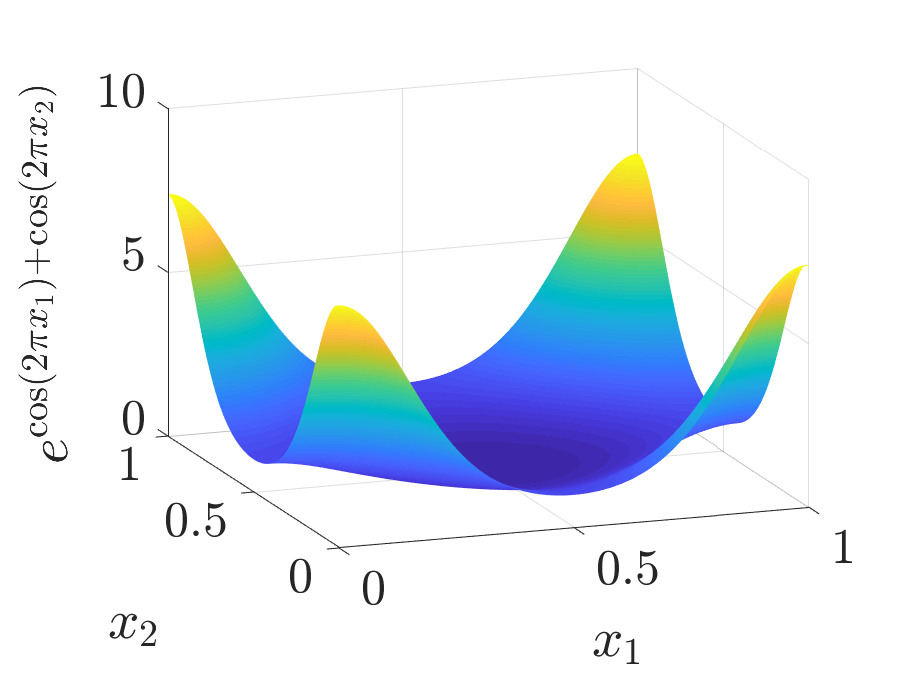
\includegraphics[width=\textwidth]{ExpCos}
%\includegraphics[width=\textwidth]{example}
\end{subfigure}
\caption{Exp(Cos) in 2 dimensions}
\label{fig:Exp(Cos)}
\end{figure}
%\vspace{-3ex}
where the function is defined as
\begin{align*}
\begin{matrix}
f(\vx) &= e^{\sum_{i=1}^d\cos(2 \pi x_d)},  
\\
\\
\int_{[0,1]^d} f(\vx) \dvx &= \text{BesselI(0,1)}^d
\end{matrix}
\end{align*}
where `$\text{BesselI}$' is the \textit{modified Bessel} function. Exp(Cos) function is periodic in $[0,1]$, so we do not need to use any \textit{transform} to make it periodic.







\item Keister function

The following multidimensional integral example is based on the paper \cite{KeisterExample}, inspired by a physics application.


\begin{figure}[H]
\linespread{0.7}
\centering
\captionsetup[subfigure]{labelformat=empty}
\begin{subfigure}[b]{0.48\textwidth}
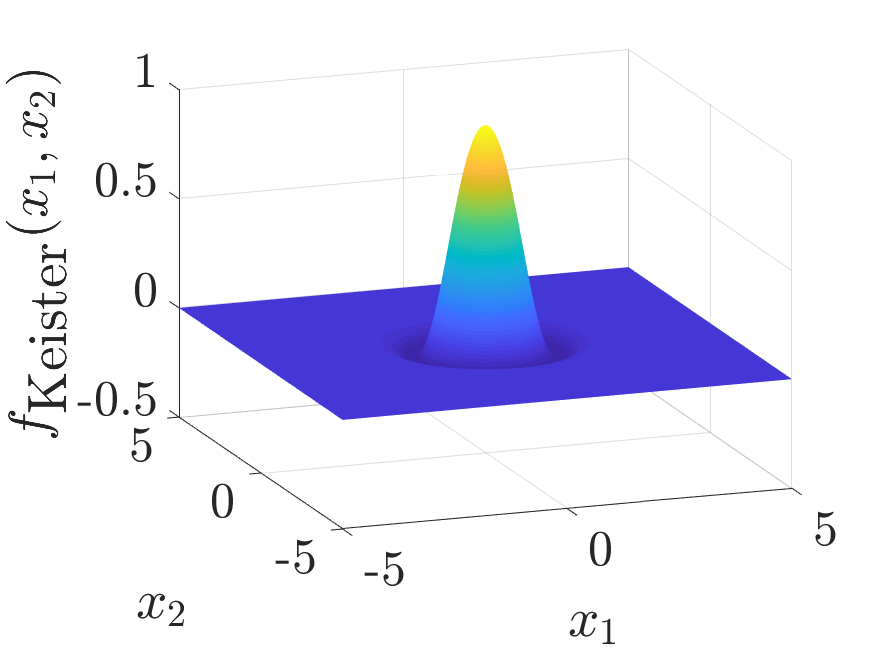
\includegraphics[width=\textwidth]{Keister_wholeR}
%\includegraphics[width=\textwidth]{example}
\end{subfigure}
\centering
\captionsetup[subfigure]{labelformat=empty}
\begin{subfigure}[b]{0.48\textwidth}
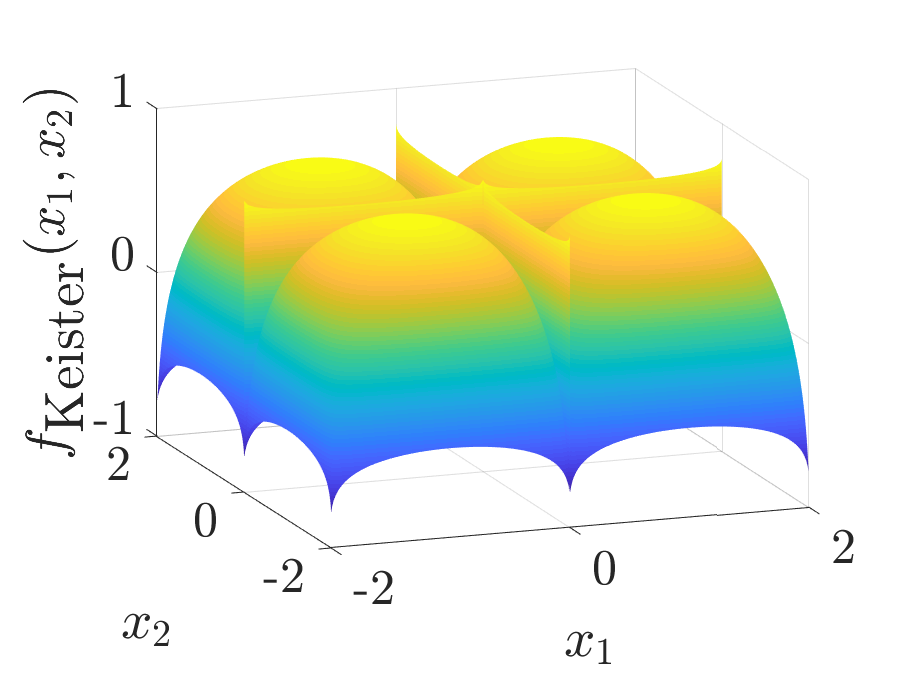
\includegraphics[width=\textwidth]{Keister_cube}
%\includegraphics[width=\textwidth]{example}
\end{subfigure}
\caption{Keister function in original form and its transform to $[0,1]^2$}
\label{fig:Keister}
\end{figure}


\begin{align*}
f(\vx) &=  \cos(\norm{ \vx}) \exp(-\norm{ \vx }^2) \dvx, \;  
\\
\\
\int_{\mathbb{R}^d} f(\vx) \dvx & = \frac{2 \pi^{\frac d2}}{\text{gamma}(\frac d2)} \text{cosinteg}(d), \quad d=1,2,3,\hdots
\end{align*}
where

\begin{align*}
\text{cosinteg}(1) &= \frac{\sqrt{\pi}}{2 \exp(1/4)}
\\
\text{sininteg}(1) &= \int_{x=0}^\infty \exp(-\vx^T\vx)\sin(\vx) \dvx \quad = \quad 0.4244363835020225
\\
\text{cosinteg}(2) &= \frac{1-\text{sininteg}(1)}{2}
\\
\text{sininteg}(2) &= \frac{\text{cosinteg}(1)}{2}
\\
\text{cosinteg}(j) &= \frac{(j-2)\text{cosinteg}(j-2)-\text{sininteg}(j-1)}{2},
\quad j =3,4,\hdots
\\
\text{sininteg}(j) &= \frac{(j-2)\text{sininteg}(j-2)-\text{cosinteg}(j-1)}{2},
\quad j =3,4,\hdots
\\
\text{where gamma(.)} & := \text{gamma function}
% ref: https://www.mathworks.com/help/matlab/ref/gamma.html
\end{align*}












\item Multivariate Normal




We use the Genz's method to compute Multivariate normal probability as explained below. This method reduces the original dimension of the problem by 1.


\begin{figure}[H]
\linespread{0.7}
\centering
\captionsetup[subfigure]{labelformat=empty}
\begin{subfigure}[b]{0.48\textwidth}
%\includegraphics[width=\textwidth]{example}
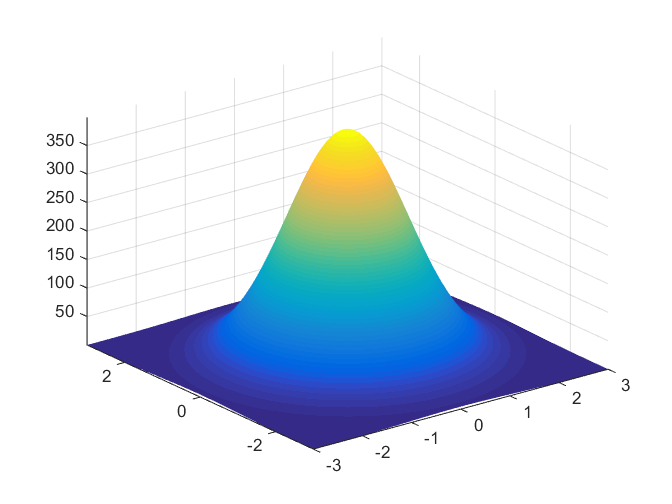
\includegraphics[width=\textwidth]{Plotting_gaussian}
\end{subfigure}
\centering
\begin{subfigure}[b]{0.48\textwidth}
%\includegraphics[width=\textwidth]{example}
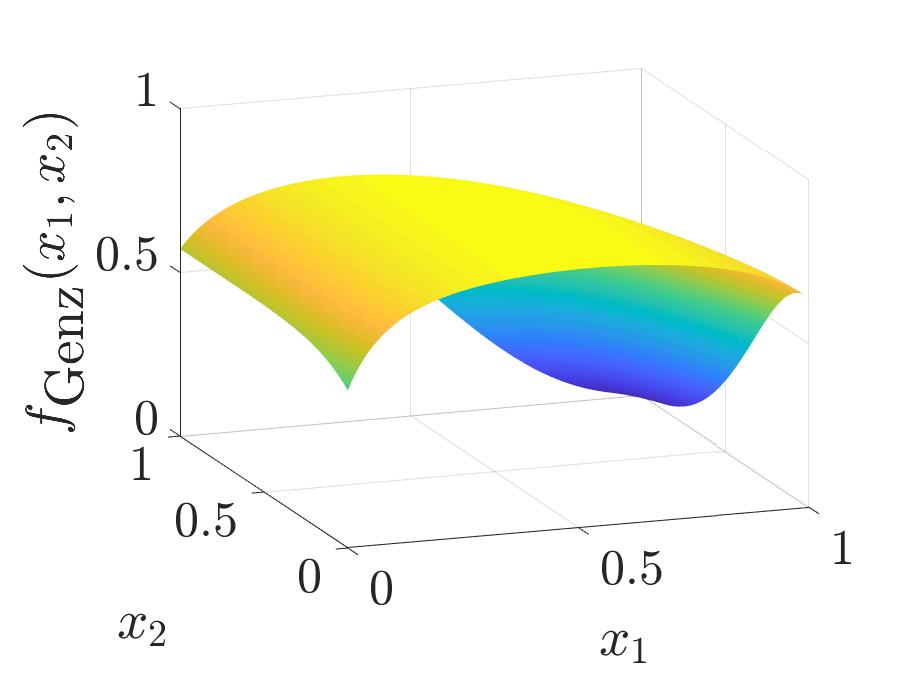
\includegraphics[width=\textwidth]{GenzFun}
\end{subfigure}
\caption{Mutivariate Normal and Genz function }
\label{fig:MVN and Genz}
\end{figure}
\begin{tabular}{m{8.5cm}m{3cm}}
%{Multivariate Normal (MVN)} \vspace{-2ex}
\begin{gather*}
\mu = \int_{[\va,\vb] \in \mathbb{R}^d} \frac{\exp\bigl(- \frac 12 \vt^T \mSigma^{-1} \vt \bigr)}{\sqrt{(2 \pi)^d \det(\mSigma)}} \, \dvt \
\overset{\text{\small\cite{Gen93}}}{=} \ 
\int_{[0,1]^{d-1}} f_{\text{Genz}}(\vx) \, \dvx 
\end{gather*} 
% & 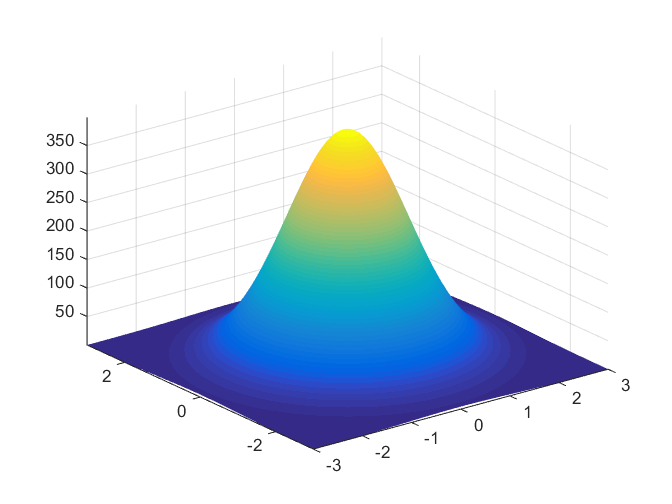
\includegraphics[width=3cm,angle=0]{Plotting_gaussian.png}
\end{tabular}

where $\mSigma= \mL \mL^T$ is the Cholesky decomposition of the covariance matrix, $\mL = (l_{jk})_{j,k=1}^d$ is a lower triangular matrix, and

\begin{align*}
\valpha_1 &= \Phi(a_1), \quad \vbeta_1 = \Phi(b_1)
\\
\valpha_j(x_1,...,x_{j-1}) &= \Phi
\left(
\frac{1}{l_{jj}} 
\left(
a_j - \sum_{k=1}^{j-1} l_{jk} \Phi^{-1}(\valpha_k + x_k(\vbeta_k-\valpha_k))
\right)
\right), j=2,...,d,
\\
\vbeta_j(x_1,...,x_{j-1}) &= \Phi
\left(
\frac{1}{l_{jj}} 
\left(
b_j - \sum_{k=1}^{j-1} l_{jk} \Phi^{-1}(\valpha_k + x_k(\vbeta_k-\valpha_k))
\right)
\right), j=2,...,d,
\\
\\
f_{\text{Genz}}(\vx) &= \prod_{j=1}^d [\vbeta_j(\vx) - \valpha_j(\vx)]
\end{align*}

As we see from the figure, Genz function is not periodic, So we need to make it periodic to get the best accuracy with Bayesian cubature.


We use the following parameter values for the numerical examples
\begin{equation*}
\begin{array}{c|ccc}
 & a  & b & L  \\
\hline
d=2 
 & 
\begin{pmatrix}
-6 \\ -2 \\ -2
\end{pmatrix}
 & 
\begin{pmatrix}
5 \\ 2 \\ 1
\end{pmatrix} 
 & 
\begin{pmatrix}
4 & 1 & 1 \\ 0 & 1 & 0.5 \\ 0 & 0 & 0.25
\end{pmatrix} 
\\
d=3
 & 
\begin{pmatrix}
-6 \\ -2 \\ -2 \\ 2
\end{pmatrix}
 & 
\begin{pmatrix}
5 \\ 2 \\ 1 \\2
\end{pmatrix} 
 & 
\begin{pmatrix}
4 & 1 & 1 & 1\\ 0 & 1 & 0.5 & 0.5 \\ 0 & 0 & 0.25 & 0.25 \\ 0 & 0 & 0 & 0.25
\end{pmatrix} 
\end{array}
\end{equation*}

%\begin{equation*}
%\begin{array}{ccccc}







\item Option pricing


The price of financial derivatives can often be modeled by high dimensional integrals. If the underlying asset is described in terms of a Brownian motion, B, at time $t_1,...,t_d$, then $Z = (B(t_1), ..., B(t_d)) \sim \mathcal{N}(\vzero,\mSigma)$, where $\mSigma = \left(\min(t_j,t_k) \right)_{j,k=1}^d$, and the fair price of the option is

\begin{align*}
\mu = \int_{\mathbb{R}^d} \text{payoff}(\vz) \frac{\exp(\frac 12 \vz^T\mSigma^{-1}\vz)}{\sqrt{(2\pi)^d \det(\mSigma)}} \dvz = \int_{[0,1]^d} f(\vx) \dvx
\end{align*}
where the function payoff(.) describes the discounted payoff of the option,


\begin{align*}
f(\vx) = \text{payoff}(\vz), & \quad \vz = \mL 
\begin{pmatrix}
\Phi^{-1}(x_1) \\ \vdots \\ \Phi^{-1}(x_d)
\end{pmatrix},
\end{align*}
and $\mL$ is any square matrix satisfying $\mSigma = \mL \mL^T$.

For the Asian arithmetic mean call option

\begin{align*}
\text{payoff}(\vz) = \max\left( \frac 1d  \sum_{j=1}^d S_j - K, 0 \right) e^{-r t}, \quad
S_j = S_0 \exp((r-\sigma^2/2)t_j + \sigma z_j )
\end{align*}
where $d$ - number of dimensions and $T, S, S_0, K, r, \sigma$ are the parameters to be specified


\end{enumerate}




































\section{Conclusion}


We developed a generalized technique of \emph{Fast transform kernel}. Using this technique, further developed fast automatic Bayesian cubature algorithm that takes very low computational cost in the order of $\Order(n \log n)$ comparing to direct Bayesian cubature of $\Order(n^{3})$, so it can be used in practical applications. 
By adjusting the Bernoulli order $r$ of the kernel and using the appropriately smoother variable transformation, we could get 
%$\Order(n^{-2})$ and $\Order(n^{-4})$
higher order of error convergence when the integrand is assumed to have zero mean. 
In general case without any assumption on the integrand mean
%When the integrand is assumed to have arbitrary mean $m \neq 0$ case
, the optimal $\hmu$ is just the sample mean and so the order of convergence is defined by how smoother the underlying function being integrated and the variable transformation being used. 
Though the optimal $\hmu$ is just the sample mean, the error bound $\errn$ still depends on the kernel order.
So when we use higher order $r$, the error bound $\errn$ closely matches the actual error.
We could use the algorithm to integrate upto $2^{23}$ data points on a 16GB of RAM memory and i7-3630QM computer within 5 minutes. 
Numerical results show that the theoretical error $\errn$ closely matches the actual error but it could still be improved with more tighter error bound especially when the $r$ is smaller.





\section{Future work}
As an extension to the ideas and techniques established in this work, the following are considered potential future work

\begin{enumerate}


\item Sobol points and Fast Walsh Transform (FWT)

We have shown one example of a special form of kernel with defined requirements to build a \textit{Fast transform kernel}.
Using the established generalized requirements for a {fast-transform-kernel}, we could use the same approach with other kernels with suitable point-sets to achieve similar or better performance and accuracy. One such point-sets that to consider in future is, \textit{Sobol points} and with appropriate choice of kernel, which should lead to \textit{Fast Walsh Transform}.

\item Control variates

We would like to approximate a function of the form
$ (f - \beta_1 g_1 -, ... , - \beta_p g_p) $

than
\begin{align*}
f = \mathcal{N} \left( \beta_0 + \beta_1 g_1 + , ... , + \beta_p g_p, s^2 \mC  \right)
\end{align*}

\item Function approximation

Let us consider approximating a function of the form
\begin{align*}
\int_{[0,1]^d} \underbrace{ f(\vphi(\vt)) . \abs{\frac{\partial \vphi}{\partial \vt}} }_{g(\vt)} \dvt
\end{align*}
where $\abs{\frac{\partial \vphi}{\partial \vt}}$ is Jacobian and then

\begin{align*}
g(\vpsi(\vx)) &= f( \underbrace{ \vphi(\vpsi(\vx) }_{\vx } ) . \abs{\frac{\partial \vphi}{\partial \vt} }  (\vpsi(\vx))
\\
f(\vx) &= g(\vpsi(\vx)) . \frac{1}{  \abs{\frac{\partial \vphi}{\partial \vt}}  (\vpsi(\vx)) }
\end{align*}
Finally, the function approximation is

\begin{align*}
\tilde{f}(\vx) &= \tilde{g}(\vpsi( \vx )) \\
&= \sum w_i C(.,.)
\end{align*}

\item Deterministic interpretation of Bayesian cubature

\end{enumerate}











\iffalse

% For one-column wide figures use
\begin{figure}
% Use the relevant command to insert your figure file.
% For example, with the graphicx package use
  \includegraphics{example.eps}
% figure caption is below the figure
\caption{Please write your figure caption here}
\label{fig:1}       % Give a unique label
\end{figure}
%
% For two-column wide figures use
\begin{figure*}
% Use the relevant command to insert your figure file.
% For example, with the graphicx package use
  \includegraphics[width=0.75\textwidth]{example.eps}
% figure caption is below the figure
\caption{Please write your figure caption here}
\label{fig:2}       % Give a unique label
\end{figure*}
%
% For tables use
\begin{table}
% table caption is above the table
\caption{Please write your table caption here}
\label{tab:1}       % Give a unique label
% For LaTeX tables use
\begin{tabular}{lll}
\hline\noalign{\smallskip}
first & second & third  \\
\noalign{\smallskip}\hline\noalign{\smallskip}
number & number & number \\
number & number & number \\
\noalign{\smallskip}\hline
\end{tabular}
\end{table}

\fi



%\begin{acknowledgements}
%If you'd like to thank anyone, place your comments here
%and remove the percent signs.
%\end{acknowledgements}

% BibTeX users please use one of
%\bibliographystyle{spbasic}      % basic style, author-year citations
%\bibliographystyle{spmpsci}      % mathematics and physical sciences
%\bibliographystyle{spphys}       % APS-like style for physics
%\bibliography{}   % name your BibTeX data base
\bibliography{mybib}
\bibliographystyle{alpha}

% Non-BibTeX users please use
\begin{thebibliography}{}
%
% and use \bibitem to create references. Consult the Instructions
% for authors for reference list style.
%
\bibitem{RefJ}
% Format for Journal Reference
Author, Article title, Journal, Volume, page numbers (year)
% Format for books
\bibitem{RefB}
Author, Book title, page numbers. Publisher, place (year)
% etc
\end{thebibliography}


\end{document}
% end of file template.tex